% Adapted from the official IEEE Conference Template, IEEE / Overleaf.
% Main document: main.tex. Compiler: pdfLaTeX.
\documentclass[conference,a4paper]{IEEEtran}
\usepackage[T1]{fontenc}
\usepackage{cite}
\usepackage{amsmath,amssymb}
\usepackage{graphicx}
\usepackage{xcolor}
\usepackage{array,booktabs,tabularx}
\usepackage{tikz}
\usetikzlibrary{arrows.meta,positioning}
\usepackage{pdfpages}
\usepackage[hidelinks]{hyperref}
% EDIT THIS FILE FIRST. The default single member is only a placeholder.
% Set the actual team size (1--8). Enter members in alphabetical order.
% Copy names EXACTLY from matriculation cards. Do not invent contributions.
\newcommand{\TeamSize}{1}
\newcommand{\ReportTitle}{[Your Original Survey Title]}
\newcommand{\SubmissionDate}{[Actual submission date]}

% The same names appear on the cover and at the beginning of the body.
\expandafter\newcommand\csname MemberName1\endcsname{[Member 1 full name]}
\expandafter\newcommand\csname MemberName2\endcsname{[Member 2 full name]}
\expandafter\newcommand\csname MemberName3\endcsname{[Member 3 full name]}
\expandafter\newcommand\csname MemberName4\endcsname{[Member 4 full name]}
\expandafter\newcommand\csname MemberName5\endcsname{[Member 5 full name]}
\expandafter\newcommand\csname MemberName6\endcsname{[Member 6 full name]}
\expandafter\newcommand\csname MemberName7\endcsname{[Member 7 full name]}
\expandafter\newcommand\csname MemberName8\endcsname{[Member 8 full name]}

% Write short, factual contributions. Keep each to 2--3 short lines.
\expandafter\newcommand\csname MemberWork1\endcsname{[Actual contribution]}
\expandafter\newcommand\csname MemberWork2\endcsname{[Actual contribution]}
\expandafter\newcommand\csname MemberWork3\endcsname{[Actual contribution]}
\expandafter\newcommand\csname MemberWork4\endcsname{[Actual contribution]}
\expandafter\newcommand\csname MemberWork5\endcsname{[Actual contribution]}
\expandafter\newcommand\csname MemberWork6\endcsname{[Actual contribution]}
\expandafter\newcommand\csname MemberWork7\endcsname{[Actual contribution]}
\expandafter\newcommand\csname MemberWork8\endcsname{[Actual contribution]}

% Dates are the actual signing dates, not today's date or the deadline.
\expandafter\newcommand\csname MemberDate1\endcsname{[DD/MM/YYYY]}
\expandafter\newcommand\csname MemberDate2\endcsname{[DD/MM/YYYY]}
\expandafter\newcommand\csname MemberDate3\endcsname{[DD/MM/YYYY]}
\expandafter\newcommand\csname MemberDate4\endcsname{[DD/MM/YYYY]}
\expandafter\newcommand\csname MemberDate5\endcsname{[DD/MM/YYYY]}
\expandafter\newcommand\csname MemberDate6\endcsname{[DD/MM/YYYY]}
\expandafter\newcommand\csname MemberDate7\endcsname{[DD/MM/YYYY]}
\expandafter\newcommand\csname MemberDate8\endcsname{[DD/MM/YYYY]}

% Add ONLY genuine signatures personally supplied by the relevant members:
% signatures/member-1.png ... signatures/member-8.png.
% Alternatively sign the final PDF personally after content is complete.
% Never create signatures with a script, handwriting font, or AI.

\newif\ifAttachTurnitin
\AttachTurnitinfalse
% After checking the completed report, upload the authentic PDF as
% attachments/turnitin-report.pdf and change the line above to:
% \AttachTurnitintrue


\newcommand{\todo}[1]{\textcolor{blue!55!black}{[#1]}}
\newcommand{\membername}[1]{\csname MemberName#1\endcsname}
\newcommand{\memberwork}[1]{\csname MemberWork#1\endcsname}
\newcommand{\memberdate}[1]{\csname MemberDate#1\endcsname}
\newcommand{\membersignature}[1]{%
  \IfFileExists{signatures/member-#1.png}{%
    \includegraphics[width=2.6cm,height=0.65cm,keepaspectratio]{signatures/member-#1.png}%
  }{\parbox[c][0.65cm][c]{2.6cm}{\centering\scriptsize [Real signature]}}%
}
\newcommand{\MemberRow}[1]{%
  \parbox[c][0.85cm][c]{0.22\textwidth}{\membername{#1}} &
  \memberwork{#1} & \memberdate{#1} & \membersignature{#1}\\\hline
}
\newcommand{\PrintMemberRows}{%
  \MemberRow{1}%
  \ifnum\TeamSize>1 \MemberRow{2}\fi
  \ifnum\TeamSize>2 \MemberRow{3}\fi
  \ifnum\TeamSize>3 \MemberRow{4}\fi
  \ifnum\TeamSize>4 \MemberRow{5}\fi
  \ifnum\TeamSize>5 \MemberRow{6}\fi
  \ifnum\TeamSize>6 \MemberRow{7}\fi
  \ifnum\TeamSize>7 \MemberRow{8}\fi
}
\newcommand{\PrintAuthorNames}{%
  \membername{1}%
  \ifnum\TeamSize>1 , \membername{2}\fi
  \ifnum\TeamSize>2 , \membername{3}\fi
  \ifnum\TeamSize>3 , \membername{4}\fi
  \ifnum\TeamSize>4 \\ \membername{5}\fi
  \ifnum\TeamSize>5 , \membername{6}\fi
  \ifnum\TeamSize>6 , \membername{7}\fi
  \ifnum\TeamSize>7 , \membername{8}\fi
}

\begin{document}
\ifnum\TeamSize<1 \PackageError{EE6497}{TeamSize must be 1--8}{Edit config.tex}\fi
\ifnum\TeamSize>8 \PackageError{EE6497}{TeamSize must be 1--8}{Edit config.tex}\fi
\onecolumn
\thispagestyle{empty}
\begingroup
\centering
{\Large Nanyang Technological University\par}
\vspace{0.35cm}
{\large School of Electrical and Electronic Engineering\par}
\vspace{1.0cm}
{\LARGE\bfseries EE6497 Survey Report\par}
\vspace{0.35cm}
{\large Pattern Recognition and Deep Learning\par}
\vspace{0.65cm}
{\normalsize Submission date: \SubmissionDate\par}
\endgroup

\vspace{0.8cm}
\noindent{\large\bfseries Statement of Originality}\par
\vspace{0.25cm}
\noindent I hereby certify that the work embodied in this report is the result of original research and is free of plagiarised materials.

\vspace{0.55cm}
\noindent\textbf{Team members, contributions and signatures}\par
\vspace{0.2cm}
\noindent Names must match matriculation cards exactly and appear in alphabetical order. Each member signs and dates their own row.
\vspace{0.3cm}

\begingroup
\small
\setlength{\tabcolsep}{5pt}
\renewcommand{\arraystretch}{1.15}
\noindent\begin{tabularx}{\textwidth}{|>{\raggedright\arraybackslash}p{0.22\textwidth}|>{\raggedright\arraybackslash}X|>{\raggedright\arraybackslash}p{0.16\textwidth}|>{\centering\arraybackslash}p{0.17\textwidth}|}
\hline
\textbf{Full name} & \textbf{Contribution} & \textbf{Date signed} & \textbf{Signature} \\ \hline
\PrintMemberRows
\end{tabularx}
\endgroup

\vspace{0.35cm}
\noindent{\footnotesize\itshape Template fields are unsigned. Sign only after reviewing the completed report.}
\vfill
\noindent{\footnotesize\color{black!65}Template setup: set the actual team size (1--8) and all member fields in \texttt{config.tex}. Remove this setup note before submission.}

% \twocolumn starts a new physical page. Do not reset the page counter.
\twocolumn
\pagestyle{plain}
\title{\ReportTitle}
\author{\IEEEauthorblockN{\PrintAuthorNames}
\IEEEauthorblockA{School of Electrical and Electronic Engineering\\
Nanyang Technological University, Singapore}}
\maketitle
\thispagestyle{plain}
\begin{abstract}
\todo{Replace this with an original abstract stating the survey topic, scope, organizing perspective, main synthesis and future directions. Write it after reviewing the literature. This template contains no research findings.}
\end{abstract}

\begin{IEEEkeywords}
\todo{Topic keyword}, \todo{method keyword}, literature survey
\end{IEEEkeywords}

\section{Introduction}
\todo{Define a focused problem in pattern recognition or deep learning. Explain its importance using verified sources, set the survey boundaries, and state the questions this report will answer. Use an original title that differs from existing papers.}

\todo{Describe how this survey organizes and compares the literature. Replace every blue instruction and bracketed field before submission. Do not present these prompts as completed research.}

\section{Scope and Literature Selection}
\todo{Record the actual search sources, search terms, search date, publication period, and inclusion/exclusion criteria. Focus on recent work (approximately the last three years) from the venues specified in the instructor email. Check existing surveys and explain how your scope differs. Do not invent a search process or paper count.}

\section{Background and Taxonomy}
\todo{Define every reused acronym and each mathematical symbol at first appearance. Explain necessary concepts in your own words with appropriate citations. Develop a taxonomy justified by the papers you read. Fig.~\ref{fig:taxonomy} is an editable structural example; replace its categories and relationships with your own synthesis.}

% Original editable TikZ placeholder, created for this project.
% This is a structure example, NOT a completed research taxonomy.
\begin{figure}[!b]
\centering
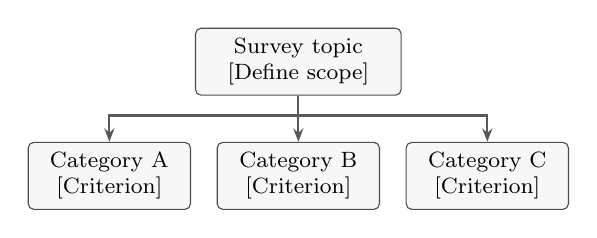
\begin{tikzpicture}[
  box/.style={draw=black!70,rounded corners=2pt,align=center,
    font=\footnotesize,minimum height=0.85cm,text width=1.85cm,
    inner sep=3pt,fill=black!3},
  link/.style={-{Stealth[length=1.7mm]},thick,draw=black!65}]
  \node[box,text width=2.4cm] (topic) at (0,0) {Survey topic\\{[Define scope]}};
  \node[box] (a) at (-2.4,-1.45) {Category A\\{[Criterion]}};
  \node[box] (b) at (0,-1.45) {Category B\\{[Criterion]}};
  \node[box] (c) at (2.4,-1.45) {Category C\\{[Criterion]}};
  \draw[link] (topic.south) -- ++(0,-0.25) -| (a.north);
  \draw[link] (topic.south) -- (b.north);
  \draw[link] (topic.south) -- ++(0,-0.25) -| (c.north);
\end{tikzpicture}
\caption{Original editable taxonomy layout. Placeholder categories and links must be replaced with a literature-supported synthesis. No research conclusion is represented.}
\label{fig:taxonomy}
\end{figure}


\section{Comparative Analysis}
\todo{Compare approaches using a consistent set of criteria. Identify the exact method in each reviewed work and distinguish a newly proposed model from an applied or used existing model. Discuss assumptions, evidence, results and trade-offs across papers. Table~\ref{tab:evidence} provides an original editable layout, with no invented sources or measurements.}

% Original editable table structure. Add verified sources and real evidence.
\begin{table}[!t]
\caption{Editable evidence matrix: all entries are placeholders}
\label{tab:evidence}
\centering
\footnotesize
\setlength{\tabcolsep}{3pt}
\renewcommand{\arraystretch}{1.2}
\begin{tabularx}{\columnwidth}{@{}>{\raggedright\arraybackslash}p{0.18\columnwidth}*{3}{>{\raggedright\arraybackslash}X}@{}}
\toprule
Source & Main idea & Evidence / setting & Limitation \\
\midrule
{[Citation]} & [Describe] & [Verify] & [Discuss] \\
{[Citation]} & [Describe] & [Verify] & [Discuss] \\
{[Citation]} & [Describe] & [Verify] & [Discuss] \\
\bottomrule
\end{tabularx}
\end{table}


\todo{When reproducing a reported number, cite its actual source and retain the dataset, evaluation protocol, metric definition and units. Distinguish reported results from your own experiments, if any. Avoid treating incomparable settings as a valid ranking.}

\section{Learning Points and Future Directions}
\todo{Synthesize what the reviewed evidence teaches. Explain agreement and disagreement across studies, identify specific open questions, and propose future research with a rationale grounded in the survey. Distinguish your proposals from established results.}

\section{Conclusion}
\todo{Answer the survey questions and summarize the supported takeaways. Do not introduce claims or citations that have not been discussed.}

\section*{Template reference example}
The instructor recommends the survey by Ker et al.~\cite{ker2018medical} as a writing example. This citation demonstrates IEEE bibliography formatting; it does not select a topic or supply findings for this report. Replace this paragraph with your own discussion and retain only references actually used.

% Add acknowledgments / AI-use disclosure only when appropriate and factual,
% following the current NTU guidelines and any course instructions.
% Do not add fictitious funding or author contributions.


% The live entry is the instructor's authentic example survey.
% Replace the demo citation and .bib entry with verified literature.
\bibliographystyle{IEEEtran}
\bibliography{references}

\clearpage
\onecolumn
\ifAttachTurnitin
  \IfFileExists{attachments/turnitin-report.pdf}{%
    \includepdf[pages=-,pagecommand={\thispagestyle{plain}}]{attachments/turnitin-report.pdf}%
  }{%
    \PackageError{EE6497}{Turnitin attachment is enabled but the PDF is missing}
    {Upload attachments/turnitin-report.pdf or set AttachTurnitinfalse in config.tex}%
  }
\else
  \thispagestyle{plain}
\raggedright
\section*{Turnitin Report Attachment Placeholder}
\noindent\textbf{No Turnitin report is attached to this template.}
\vspace{0.4cm}

\noindent After completing the survey, obtain and review the authentic Turnitin report. Save it as \texttt{attachments/turnitin-report.pdf}, then set \texttt{\string\AttachTurnitintrue} in \texttt{config.tex}. Recompile to append all pages after the references. This placeholder page will disappear automatically.

\vspace{0.4cm}
\noindent If your Turnitin export cannot be included by the compiler, download the completed survey PDF and append the authentic Turnitin PDF with a PDF merger. Preserve the order: signed cover, IEEE body and references, Turnitin report.

\vspace{0.4cm}
\noindent Check the combined PDF before submitting it to NTULearn. Do not submit this placeholder page as a Turnitin report, and do not invent a similarity score.


\vspace{0.4cm}
\noindent The instructor permits a screenshot of the overlap-score page only if the complete Turnitin report cannot be appended. Convert that authentic screenshot to a one-page PDF using the same filename and enable the attachment. There is no acceptable similarity-score threshold: inspect the highlighted passages and revise copied sentences.

\fi
\end{document}
